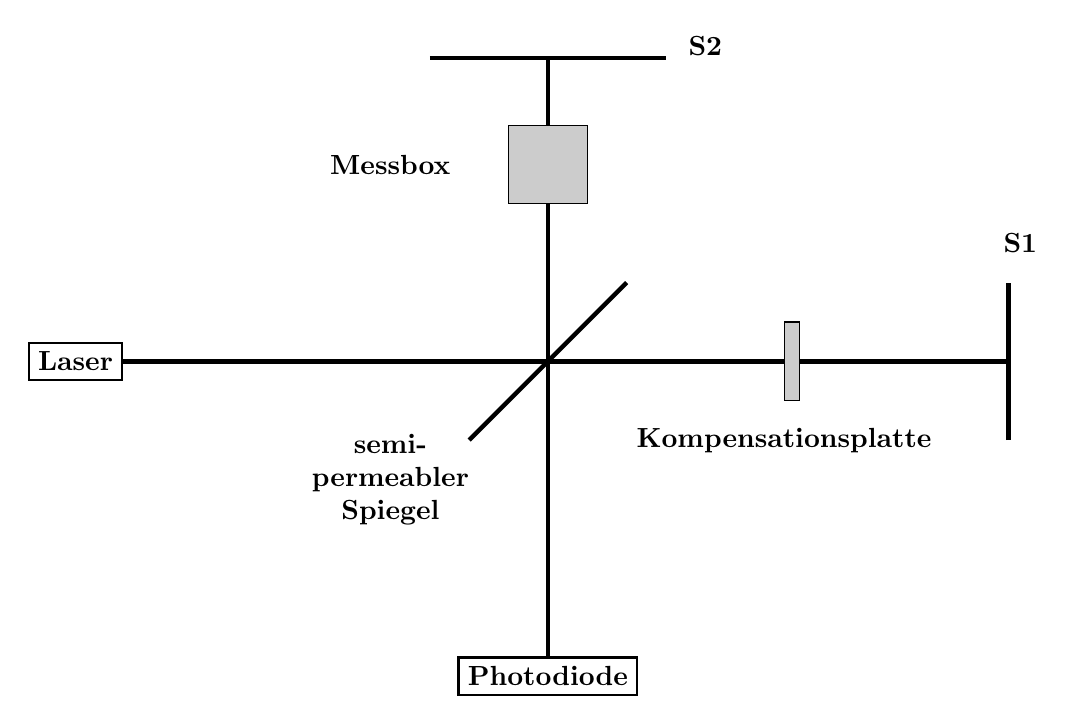
\begin{tikzpicture}
	\node(LASER)at(-6,0)[rectangle,draw,thick]{\textbf{Laser}};
	\node(center)at(0,0){};
	\node(S1)at(6,0){};
	\node(S2)at(0,4){};
	\node(D)at(0,-4)[rectangle,draw,thick]{\textbf{Photodiode}};

%Beschriftung	
	\node(hdl)at(-2,-1.5)[align=center]{\textbf{semi-}\\\textbf{permeabler}\\ \textbf{Spiegel}};
	\node(Box)at(-2,2.5){\textbf{Messbox}};.5
	\node(K)at(3,-1){\textbf{Kompensationsplatte}};
	\node(Spiegel2)at(2,4){\textbf{S2}};
	\node(Spiegel1)at(6,1.5){\textbf{S1}};
	
	\path [-, ultra thick]
	(-1,-1)edge(1,1)            % semipermeabler Spiegel
	(LASER)edge(S1)             % Strahlengang
	(S2)edge(D)                 % Strahlengang
	(-1.5,3.85)edge(1.5,3.85)   % Spiegel 2
	(5.85,-1)edge(5.85,1);      % Spiegel 1
	\filldraw[fill=gray!40!white,draw=black](-0.5,3)rectangle(0.5,2);
	\filldraw[fill=gray!40!white,draw=black](3,0.5)rectangle(3.2,-0.5);
\end{tikzpicture}